\section{Cooperative coevolution of morphologically heterogeneous robots \cite{gomes2015cooperative}}

\begin{frame}{Problem Description}

\begin{figure}

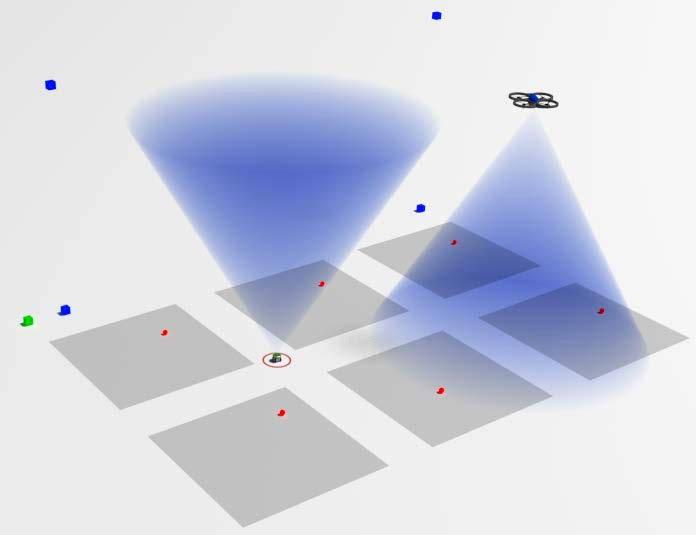
\includegraphics[width=0.8\textwidth]{gomes-fig-1}

\caption{
Figure 1 from \cite{gomes2015cooperative}.
}

\end{figure}

\end{frame}

\begin{frame}{Problem Description}

{\Large
\textbf{minimal prerequisite for meaningful cooperation}
}

\vspace{1ex}

\begin{columns}
\begin{column}{0.02\textwidth}
\end{column}
\begin{column}{0.02\textwidth}
\Huge
\[
\bm{\Bigg\Updownarrow}
\]
\end{column}
\begin{column}{0.96\textwidth}
\begin{itemize}
\item[] \textit{Fix-Tog} --- Fixed altitude, start together
\item[] \textit{Fix-Sep} --- Fixed altitude, start separate
\item[] \textit{Var-Tog} --- Variable altitude, start together
\item[] \textit{Var-Sep} --- Variable altitude, start separate
\end{itemize}
\end{column}
\end{columns}

\vspace{1ex}

{\Large
\textbf{difficult prerequisite for meaningful cooperation}
}

\end{frame}

\begin{frame}{Treatments}

\Large
\begin{itemize}
\item \textit{Base} ---  base CCEA
\item \textit{Inc} --- incremental evolution
\item \textit{NInc} --- non-cooperative incremental evolution
\item \textit{NS} --- novelty-driven coevolution
\end{itemize}
\end{frame}

\begin{frame}{Results}

\begin{figure}
\begin{columns}
\begin{column}{0.5\textwidth}
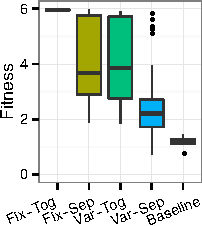
\includegraphics[width=\textwidth]{gomes-fig-2-b}
\end{column}
\begin{column}{0.5\textwidth}
\caption{
Right column of Figure 2 from \cite{gomes2015cooperative}.
}
\end{column}
\end{columns}
\end{figure}

\end{frame}

\begin{frame}{Results}

\begin{figure}

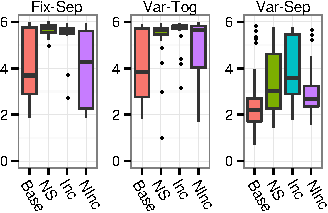
\includegraphics[width=\textwidth]{gomes-fig-3-b}

\caption{
Right column of Figure 3 from \cite{gomes2015cooperative}.
}

\end{figure}

\end{frame}

\begin{frame}{Discussion}

more difficult conditions (\textit{Fix-Sep}, \textit{Var-Tog},\textit{Var-Sep}) nicely illustrate context-dependence issue
\begin{itemize}
\item \textit{NInc} treatment: evolvability constraints + context-dependence
\end{itemize}

generalizable to other problem domains (in principle)

weakness: need to know expected cooperating roles \textit{a priori}

weakness: as number of cooperating roles increases, method becomes more computationally expensive

\end{frame}
